\documentclass[]{solarphysics}

\usepackage[hyperref,optionalrh,showbiblabels]{spr-sola-addons} % For Solar Physics 

\usepackage{graphicx}        % For eps figures, newer & more powerfull
\usepackage{amssymb}        % useful mathematical symbols
\usepackage{color}           % For color text: \color command
%\usepackage{breakurl}        % For breaking URLs easily trough lines
\def\UrlFont{\sf}            % define the fonts for the URLs

\usepackage{natbib}
\usepackage{acronym}

\usepackage{contour}
\usepackage{color}
\usepackage{tikz}
\usepackage[caption=false]{subfig}





\bibliographystyle{spr-mp-sola}





%Journal commands from AAStex
\newcommand\procspie{\ref@jnl{Proc.~SPIE}}%      % Proceedings of the SPIE 
\newcommand\apj{\ref@jnl{ApJ}}%    % Astrophysical Journal 
\newcommand\apjl{\ref@jnl{ApJL}}     % Astrophysical Journal, Letters 
\newcommand\apjs{\ref@jnl{ApJS}}%    % Astrophysical Journal, Supplement 

\newcommand{\cck}[1]{{\color{red} CCK: #1}} % CCK comment

\newcommand{\jdp}[1]{{\color{blue} JDP: #1}} % JDP comment


\begin{document}
\begin{article}
\begin{opening}

\title{Determining the Spectral Content of MOSES Images}

\author[addressref={aff1},corref,email={jacob.parker3@montana.edu}]{\inits{J.D.}\fnm{Jacob D.}~\lnm{Parker}}%\sep
\author[addressref=aff1,email={Want to include your email Charles?}]{\inits{C.C.}\fnm{Charles C.}~\lnm{Kankelborg}}%\sep
\address[id=aff1]{Montana State University}




\begin{abstract}

\end{abstract}
\keywords{Need to look through the list of allowed keywords and pick a couple}
\end{opening}

\section{Introduction}
%Cosie as possible broad scientific context

\subsection{Temporary Outline}	
	\begin{enumerate}
		\item Brief discussion of TR and events worth studying
		\item Cite previous studies the TR and motivate MOSES
		\item Briefly describe instrument concept but mostly cite previous works on this.
		\item Possibly cite the scientific success of Skylab overlapograms to prove the utility of this type of data.
		\item Point to EIS Slot Paper by MSSL folk
		\item Outline the rest of the paper.
		
	\end{enumerate}

	

	
%	 \cck{I like the idea of setting forth the symptoms first to motivate this study. A figure would help here. [Should we have a section called ``Data,'' that describes these features in detail? The intro could simply allude to them and say that they will be described in \S\,2.]}
%	 
%	 \jdp{I think you are right.  It might flow better if I discussed the data, features in the data, and previous work on it in an additional section. Then would the intro be simply broader scientific motivation for MOSES in general? I'll try and outline the intro and data section and we can go from there.}
%	
%
%	
%\cck{Should acknowledge that the wishbone, the limb brightening, and perhaps some other off-band sources, have been identified and discussed previously by Fox (2011 PhD Thesis) and Rust (2017 PhD Thesis). Summarize what they deduced about these features.}
%
%\jdp{Tom's thesis addressed this nicely.  No mention of off band features in either Lewis' thesis or ApJ paper.}
	
\section{Data}	
	
	The \ac{MOSES} sounding rocket launched from White Sands Missile Range on February 8th, 2006 at 18:44 UT. It recorded 27 exposures between 18:44:17 and 18:49:13 UT above 160 km in altitude.  Exposure times ranged from .25 - 24 seconds with a roughly 6 second readout time in between.  An exposure consists of three images, one for each of the three spectral orders m = -1, 0, and 1.  All data was dark subtracted and co-aligned to exposure number 13 prior to our study \citep{Fox2010,Fox2011,Rust2017}. 
	
	Of the different exposures, longer exposures are best for observing quiet sun features but are saturated near active regions.  To fill in missing saturated regions and increase signal to noise we form a single time averaged image in all three spectral orders. Saturated pixels are masked with NaNs (Not a Number) and treated as missing data. Since \ac{MOSES} observes through changing amounts of atmosphere throughout its flight we use the median of each image as a synthetic exposure time, rather than the amount of time the shutter is open. Masked data is then summed in time and divided by a total synthetic exposure time for each pixel to form a single time averaged image in each spectral order with no saturated pixels.  Figures \ref{fig:moses_super}a and \ref{fig:moses_super}b shows the m = 0 and 1 order time averaged images. 
	


	\begin{figure}
		
			\begin{tikzpicture}
				\node[inner sep=0pt] at (0,0)
				{\includegraphics[trim={0 3cm 0 3cm},clip, width = \linewidth]{super_zero}};
				\node[] at (-5.7,2.6) {a)};
			\end{tikzpicture}
		
				
		
		
			\begin{tikzpicture}
				\node[inner sep=0pt] at (0,0) {\includegraphics[trim={0 3cm 0 3cm},clip, width = \linewidth]{super_plus}};
			\node[] at (-5.7,2.6) {b)};
			\end{tikzpicture}	
		
		
		
			
			\begin{tikzpicture}
				%contour options for outlining text
				
				\contourlength{1pt} %how thick each copy is
				\contournumber{20}  %number of copies
				
				%place figure
				\node[inner sep=0pt] at (0,0)
				{\includegraphics[trim={0 3cm 0 3cm},clip, width = \linewidth]{super_pz}};
				
				%draw boxes and label
				\draw[-,green,line width=1mm]  (1.7,2.4)  rectangle (-1,1.3) node[left] {\contour{black}{\large \textcolor{green} 1}};
				\draw[-,green,line width=1mm] (-4.35,-2.3) rectangle  (-3.7,-1.5)  node[right] {\contour{black}{ \large \textcolor{green} 3}};
				\draw[-,green,line width=1mm] (4.6,0) rectangle (2,-1) node[left] {\contour{black}{\large \textcolor{green}2}};
						
				%add sub figure letter
				\node[] at (-5.7,2.6) {c)};	

			\end{tikzpicture}	
		

		
		\caption{Time averaged images for the m = 0 (a) and 1 (b) spectral orders, followed by their difference (c), m = 1 minus m = 0.  Regions one through three, boxed in green, show regions of high spectral contamination. Dark features from the m = 0 order are adjacent to white smears with pixel shifts too large to be Doppler shifts.}
		\label{fig:moses_super}
	\end{figure}

	

	Identifying solar features in the MOSES data that have undergone spectral dispersion is simple. Subtracting the m = 0 image (that contains no spectral dispersion) from either outboard order eliminates non-dispersed features. What remains are bipolar features of various spatial scales.  A feature in the principle wavelength, He\,{\sc ii} $\lambda 303.8$\AA, with a nonzero line-of-sight (LOS) velocity is translated along image rows.    MOSES has a spectral dispersion of $\approx 30$ km s$^{-1}$ pixel$^{-1}$, leading to a less than ten pixel shift for even the fastest LOS velocities in He\,{\sc ii}. This results in a bipolar feature with an obvious positive and negative counterpart that are immediately next to one another. Events like these have been studied in detail by several authors \citep{Fox2010,Rust2017,Courrier2018}.
	
	
	Features from other emission lines in the MOSES passband have shifts larger than 10 pixels and cannot be mistaken as Doppler shifted features in He\,{\sc ii}  $\lambda303.8$ \AA. A feature in Si\,{\sc xi} $\lambda$303.3\AA , the next closest line, would be shifted by 17 pixels. Si\,{\sc xi} features can be seen on the solar limb where He II has little to no contribution. The best example of this is seen in box 3 of Figure \ref{fig:moses_super}c.  Box 1 of Figure \ref{fig:moses_super}c has a large, coherent, negative feature dubbed the ``wishbone''.  The wishbone is very solar in appearance and has no obvious positive counterpart.  Close inspection reveals a white smear to its left that is likely a shifted wishbone in the plus order.  Unfortunately the positive portion of the wishbone is too blurry to quantify its shift by inspection. A previous study of these features by \citet{Rust2017} used a wavelet transform to isolate large scale features prior to taking the difference.  That procedure allowed \citet{Rust2017} to roughly identify a contribution from Mg\,{\sc vii} $\lambda$315\AA \  to regions 1 and 2 and from Si\,{\sc ix}/ Fe\,{\sc vi} $\lambda$296.1\AA \ to region 3 of Figure \ref{fig:moses_super}c, but not quantify the level of contamination.
	\begin{figure}
		
			\begin{tikzpicture}
			\node[inner sep=0pt] at (0,0)
			{\includegraphics[trim={0 4.7cm 0 3.6cm},clip, width = \linewidth]{eit_171}};
			\node[] at (-5.7,2.2) {a)};
			\end{tikzpicture}
			
			\begin{tikzpicture}
			\node[inner sep=0pt] at (0,0) {\includegraphics[trim={0 4.7cm 0 3.5cm},clip, width = \linewidth]{eit_195}};
			\node[] at (-5.7,2.2) {b)};
			\end{tikzpicture}	
		
			\begin{tikzpicture}
			\node[inner sep=0pt] at (0,0) {\includegraphics[trim={0 4.7cm 0 3.5cm},clip, width = \linewidth]{eit_284}};
			\node[] at (-5.7,2.2) {c)};
			\end{tikzpicture}	

			\begin{tikzpicture}
			\node[inner sep=0pt] at (0,0) {\includegraphics[trim={0 3cm 0 3.5cm},clip, width = \linewidth]{eit_304}};
			\node[] at (-5.7,2.6) {d)};
			\end{tikzpicture}	
		
		
		\caption{SOHO EIT Images taken closest the MOSES Launch.  Each channel has been rebinned to match MOSES angular resolution and co-aligned to the MOSES FOV}
		\label{fig:EIT}
	\end{figure}

	In support of the 2008 MOSES rocket flight the \acl{EIT} \citep[EIT:][]{EIT} on board the \ac{SOHO} captured 4 full disk EUV images, one in each of the 171 {\AA}, 195 {\AA}, 284 {\AA}, and 304 {\AA} channels (Figure \ref{fig:EIT}). Each image was first despiked via \texttt{iris\_prep\_despike.pro} with default settings and made level 1 via \texttt{eit\_prep.pro}. They were then rotated to 2006-02-08 18:47 UT, the timestamp of image 13 of the MOSES observing sequence \citep{Fox2011}, and rebinned to the MOSES angular resolution of 0.59 arcsec per pixel.  Each image was co-aligned to MOSES via the maximum cross correlation of the MOSES m = 0 time averaged image and EIT 304 \AA \ channel. At first glance one can find several similar feature in the \ac{MOSES} difference image (Figure \ref{fig:moses_super}c) and the \ac{EIT} 171, 195, and 284 images (Figure \ref{fig:EIT}a, \ref{fig:EIT}b, \ref{fig:EIT}c).  The presence of these features in \ac{MOSES} data indicates a contribution of coronal spectral lines to an otherwise transition region image.  
	
	While similarities between \ac{MOSES} difference images and \ac{EIT} images indicate the contribution of hotter lines to \ac{MOSES} He {\sc ii} data, they do not tell how much, and by which lines.  In Section \ref{sec:methods} we use cross-correlation, and a forward model of the \ac{MOSES} instrument that utilizes the EIT images from Figure \ref{fig:EIT} and Chianti \citep{Chianti1,Chianti8} to identify the contamination lines withing the MOSES passband, and the extent of their contribution to MOSES images.
	 
	
	 \jdp{Question, if I rotate an image to a specific time, do I maintain the original time stamp in Figure \ref{fig:EIT}, do I not display it at all, or do I label it with the new time it has been rotated to?}
		
	
	

\section{Methods}
\label{sec:methods}
	
 
 	
 	\subsection{Cross-Correlation}
 	\label{sec:crosscorrelation}
 	 
 	 	\begin{figure}
 	 		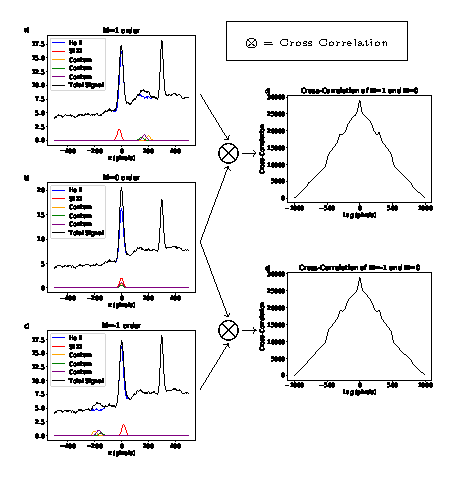
\includegraphics[scale = 1.5]{methods_fig_1.pdf}
 	 		\caption{Example 1D MOSES image in m = 1 (a), 0 (b), and -1 (c) spectral orders followed by the cross correlation of m=1 and 0 (d) and the cross-correlation of m = -1 and 0 (e).  The cross-correlation of any two MOSES orders is dominated by the autocorrelation of stationary He\,{\sc ii} features and background making them less useful in identifying spectral content.}
 	 		\label{fig:methods1}
 	 	\end{figure}
 	 	
 	 	\begin{figure}
 	 		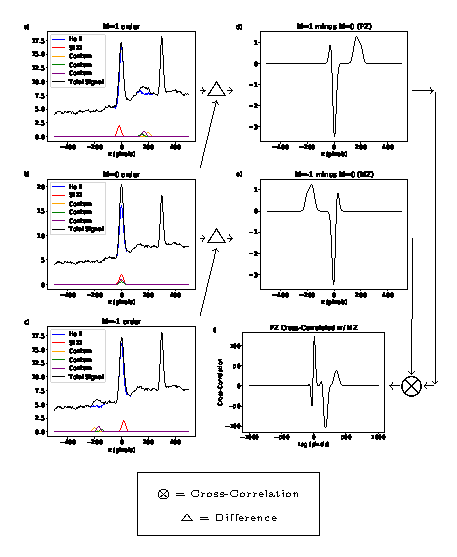
\includegraphics[scale = 1.5]{methods_fig_2.pdf}
 	 		\caption{Example 1D MOSES image in m = 1 (a), 0 (b), and -1 (c) spectral orders.  Two difference images, m=1 minus m=0 (d) and m=-1 minus m=0 (e) are cross-correlated (e).  Taking a difference removes stationary He\,{\sc ii} features so that peaks in cross-correlation are indicative of extra spectral content.  Even in this simple example one cannot read off the spectral content of the MOSES images, showing the need for a forward model.}
 	 		\label{fig:methods2}
 	 	\end{figure}
	
 	To help identify subtle pattern repetition in the MOSES difference images we cross-correlated them along the dispersion direction, or image rows.   Preforming a cross-correlation on the difference images requires justification.  An obvious first choice would have been to simply cross-correlate the m = 0 order with either outboard order.  Unfortunately the correlation function is dominated by the autocorrelation of the He\,{\sc ii} signal as seen in Figure \ref{fig:methods1}d and \ref{fig:methods1}e.  These example cross-correlations show only two noticeable peaks in correlation that are due to the auto-correlation of bright He\,{\sc ii} features, and not spectral contamination.  This would also be the case when cross-correlating the m = 1 and m = -1 order images.  By taking the difference we remove stationary He {\sc ii} objects (Figure \ref{fig:methods2}d and \ref{fig:methods2}e) and in turn their autocorrelation from the cross-correlation function (Figure \ref{fig:methods2}f).
 	
 	The cross-correlation of two difference images along their rows is defined to be,
	 	\begin{equation}
		 	P-Z \otimes M-Z = \mathcal{F}_x^{-1} \left\{\mathcal{F}_x\left(P-Z \right)*\mathcal{F}_x\left(M-Z \right)  \right\},
		 	\label{eqn:cross_correlate}
	 	\end{equation}
        
 	where $P$, $Z$, and $M$ represent the m = 1, 0 , and -1 spectral orders respectively and $\mathcal{F}_x$ is the Fast Fourier Transform (FFT) operator applied along image rows.  The MOSES image rows were also Hanning windowed, and padded with zeros, prior to applying the FFT to minimize edge effects.  The discrete Hanning window, $w(l)$, implemented was,
 	
		\begin{equation}
			w(l) = \alpha - (1-\alpha)\mathrm{cos}\left( \frac{2\pi l}{N} \right) \ \mathrm{for} \ l = 0,1,...,N-1 \quad ,
			\label{eqn:Hanning}
		\end{equation}



	where $N$ is the number of elements in the array being windowed and $\alpha = .5$.
 	
 	
 	
			 	
		\begin{figure}
		\centering
		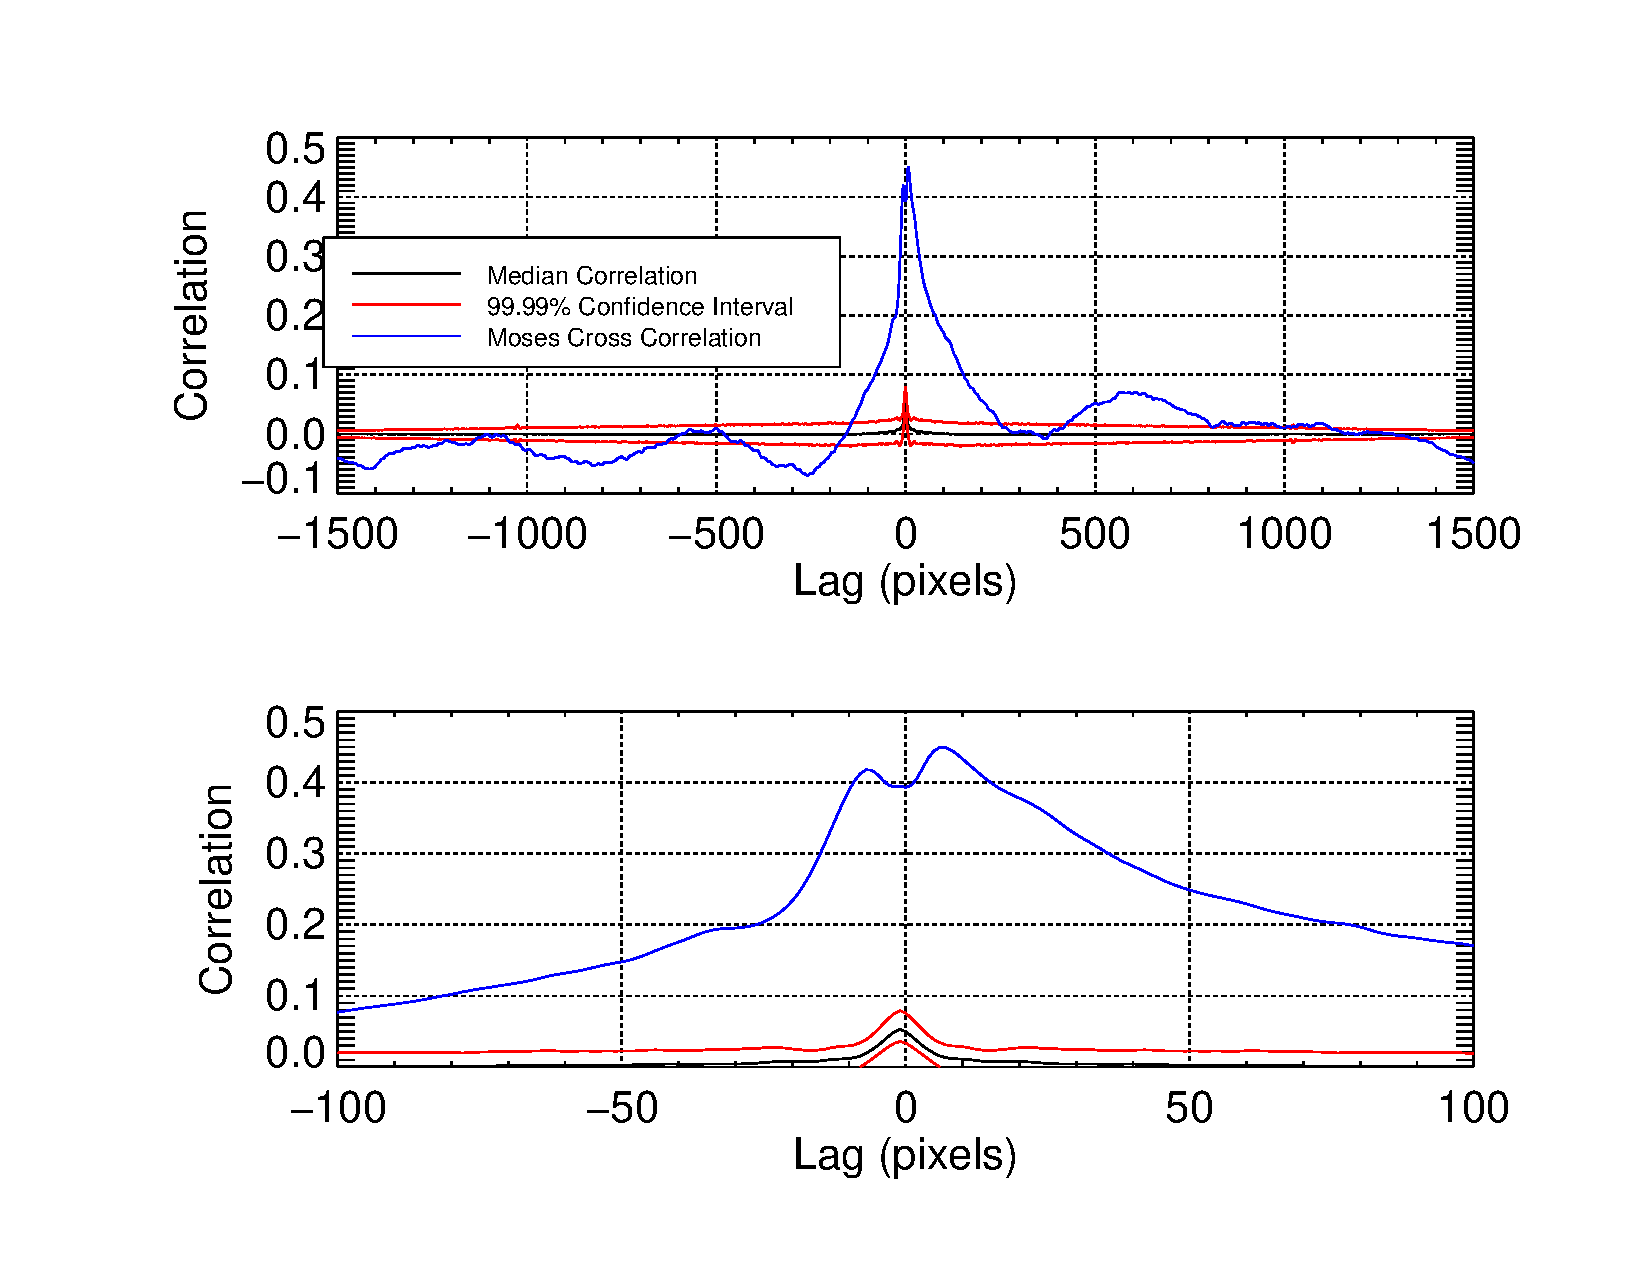
\includegraphics[width=\linewidth]{images/sigtest_5}
		\caption{The mean cross-correlation function of MOSES difference image rows (blue) overlaid on the 99.99 percent confidence interval formed by cross-correlating random data (red). }
		\label{fig:sigtest}
		\end{figure}
 	
	 This procedure yields a one dimensional cross-correlation function for each row of the MOSES difference images.  Since we are concerned mostly with bulk spectral content we then take the mean of all 1024 cross-correlation functions, one for each row, to get our final correlation curve plotted in blue in Figure \ref{fig:sigtest}. 
	 
	 The mean cross-correlation curve for the MOSES difference image has a few notable features.  There are noticeable peaks in correlation  at approximately $-800$, 250, and $+600$ pixel lags.  The largest peak in correlation, centered about zero lag, displays a double peak.   While these features are identifiable, the curve is complicated enough that quantifying peaks in correlation visually is difficult and the significance of any given peak is questionable. We therefore move to test the null hypothesis that none of these features are statistically significant by cross-correlating random data generated to match the MOSES image rows.
 
	
	\subsection{Significance Testing}
	\label{sec:sigtesting}
	The mean cross-correlation function of the two MOSES difference images, blue in Figure \ref{fig:sigtest}, has several peaks at nonzero lags.  As can be seen in Figure \ref{fig:methods2}e, these peaks can be indicative of extra spectral content.  Actual MOSES images contain information not represented in the cartoon.  Each MOSES order has a slightly different point spread function and the He\,{\sc ii} features are not all stationary.  This leads to many extra small scale features in the difference images across the field of view.  It is also unclear what magnitude of cross-correlation we should expect from extra spectral content.  We therefore move to reject the null hypothesis that the features in the MOSES difference image cross-correlation curve are the result of random correlations between each difference image and not indicative of extra spectral content.  
	
	To attempt to reject the null hypothesis we cross correlated randomly generated synthetic solar data that matched MOSES image rows in length and had similar power spectral and autocorrelation distributions.  Our test data set was generated from the MOSES image columns because they contain the same solar features as the image rows, but contain practically no spectral dispersion.  By interpolating and shuffling the elements of the MOSES columns in Fourier space we can generate a large number of test arrays for significance testing.
	
	MOSES images contain 2048 columns.  These columns have the same spatial features as MOSES image rows but with none of the spectral information.  Therefore, cross-correlating MOSES image columns will show the expected magnitude of cross-correlation from non dispersed solar features.  Despite this the MOSES image columns are insufficient for significance testing in a couple ways.  First, there is an insufficient sample size.  With features in the MOSES images ranging from four to about a hundred pixels we have at most 512 unique columns for significance testing.  Second, they are half as long as the rows, preventing us from measuring the significance of correlation past 1024 pixel lag.  Therefore we needed to generate a synthetic data set for significance testing.
	
	Using the MOSES image columns as our basis we generated $N$ random arrays that are 2048 long and match MOSES columns in both power spectral and autocorrelation distribution.  First the columns in each image, $P(x,y)$, $Z(x,y)$, and $M(x,y)$, are windowed with a Hanning window, $w(y)$(Equation \ref{eqn:Hanning}), and Fourier transformed along the column dimension, $y$.  The windowed Fourier transformed array is defined to be
	
	\begin{equation}
		\widetilde{Z}_w[x,k] = \mathcal{F}_y\left[ w(y)Z[x,y]\right], 
		\label{eqn:ztwiddle}
	\end{equation}
   
	where, $ x = 0,1,...,2047$ and $y = 0,1,...,1023$.  In Equation \ref{eqn:ztwiddle} and the following equations we will show the procedure used to generate random arrays for only the zero order, $Z(x,y)$, for simplicity even though an identical procedure was carried out on every order simultaneously.
	
	From the set of all the Fourier transformed data columns, we will generate a synthetic \emph{row}, $Z'(x)$ by populating its Fourier transform, $\widetilde{Z}'$. Each new array is formed by picking an element randomly from the distribution of Fourier transformed columns. The transformation outlined in Equation \ref{eqn:ztwiddle} gives a distribution of 511 spatial frequency bins and one DC bin that each have 1024 elements (one from each column) for each order. Once assembled, each array is further scrambled by giving each value of $k$, aside from the DC term, a random phase shift, $e^{i\phi}$.  By this method the $k^{\mathrm{th}}$ element in each new synthetic array, $\widetilde{Z}_k'$, is found as follows:
	
	\begin{equation}
		\widetilde{Z}_k^{'} = \widetilde{Z}_w\left[\sigma(m,2048), k  \right]e^{i\Phi(n)} ,
		\label{eqn:synth_array}
	\end{equation}
	where,
	
	\begin{equation}
		\sigma(m,L) = floor\{randomu(m)*L\} ,
	\end{equation}
	\begin{equation}
		\Phi(n) = 2\pi * randomu(n),
	\end{equation}
	the function $randomu()$ picks a random value from a uniform distribution between zero and one each time it is called, and $floor()$ rounds down to the nearest integer.  The function $\sigma()$ generates a random integer between zero and $L-1$.  
	
	In order create an array that is 2048 elements long from one that is 1024 elements long we require twice as many value of $k$.  We solve this problem by double picking values from the distribution for each wave number, $k$.  The values of $k$ used in Equation \ref{eqn:synth_array} are,
	
	\begin{equation}
		k_j = floor(j/2),
	\end{equation}
	where $j = 1,2,..,1022.$ Since our data is purely real we can fill in the remaining Fourier components,  negative frequencies, with the complex conjugate of the corresponding positive frequency component.  The final synthetic MOSES row is found through a FFT, 
	
	\begin{equation}
		Z' = \mathcal{F}_y^{-1}[\widetilde{Z}'].
	\end{equation}
	Again, this procedure is carried out for each order simultaneously.  To best simulate a set of three MOSES rows, one for each order, when a frequency bin is assigned a value from the distribution, the same randomly generated indices are used for each order.  For example, if the k$^{\mathrm{th}}$ frequency bin of a synthetic m = 0 order row is selected to be $\widetilde{Z}_k^{'} = \widetilde{Z}_w\left[25, k  \right]e^{i\pi}$ from the 25$^{\mathrm{th}}$ element in the distribution with a $pi$ phase shift, then the k$^{\mathrm{th}}$ element of the corresponding synthetic m = 1 and -1 rows is also  $\widetilde{P}_k^{'} = \widetilde{P}_w\left[25, k  \right]e^{i\pi}$ and  $\widetilde{M}_k^{'} = \widetilde{M}_w\left[25, k  \right]e^{i\pi}$.
	
	To verify that our N synthetic arrays match the MOSES columns we take a randomly selected 1024 element long section of each synthetic array, as well as the MOSES columns, and plot portions the power spectral and autocorrelation distributions. Figures \ref{fig:sigtestpower} and \ref{fig:sigtestauto}  show three percentiles of the distribution (10th, 50th, and 90th) for both power spectra and autocorrelation for N equal to 10,000 synthetic arrays. Figure \ref{fig:sigtestpower} shows great agreement between synthetic data and the MOSES columns in power spectral distribution.  Figure \ref{fig:sigtestauto} shows good agreement between the synthetic data and MOSES columns at the median and only marginal agreement in the wings of the distribution.  Despite that the synthetic data always has a higher autocorrelation length that the MOSES columns and therefore acts as a worse case scenario during significance testing.  
		
	\begin{figure}
		\centering
		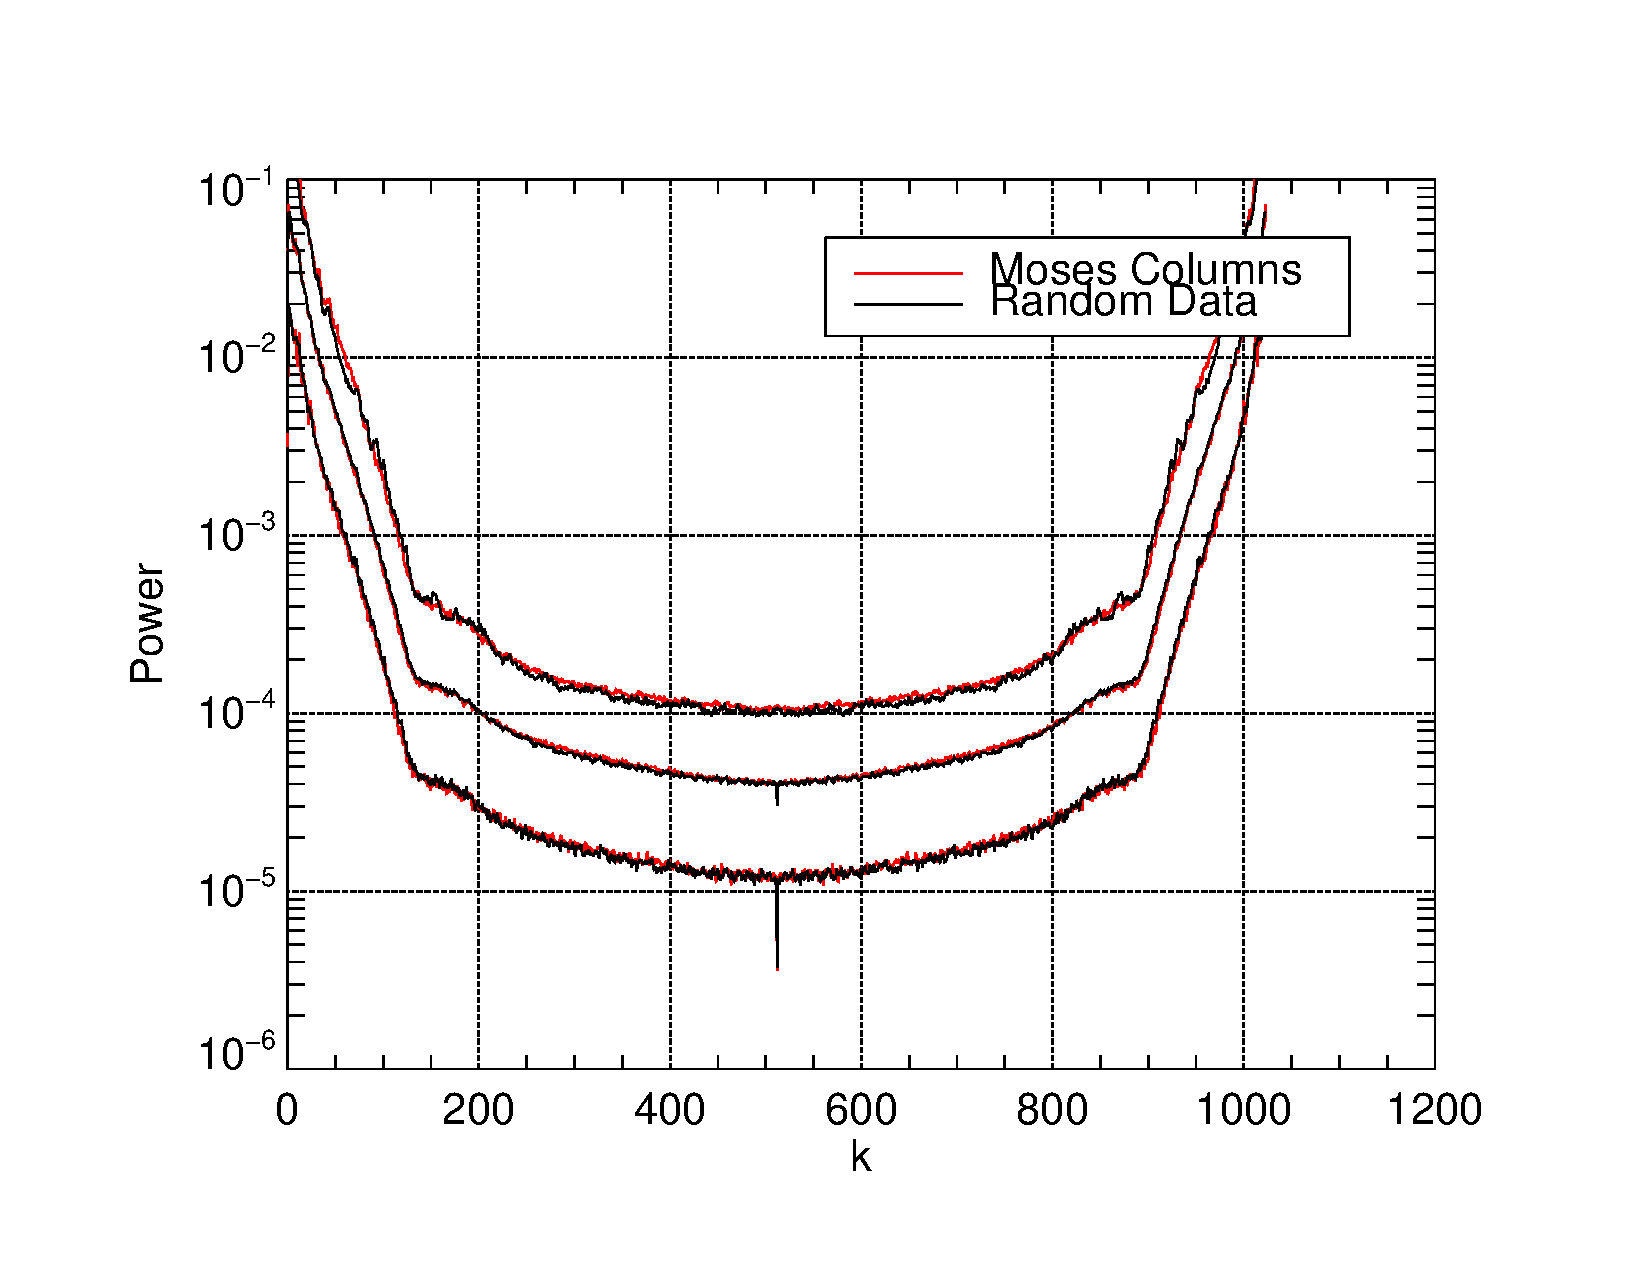
\includegraphics[width=\linewidth]{images/sigtestpower}
		\caption{The 10th, 50th, and 90th percentile of the power spectral distribution for each value of k is plotted for both the MOSES columns and synthetic data.}
		\label{fig:sigtestpower}
	\end{figure}
	\begin{figure}
		\centering
		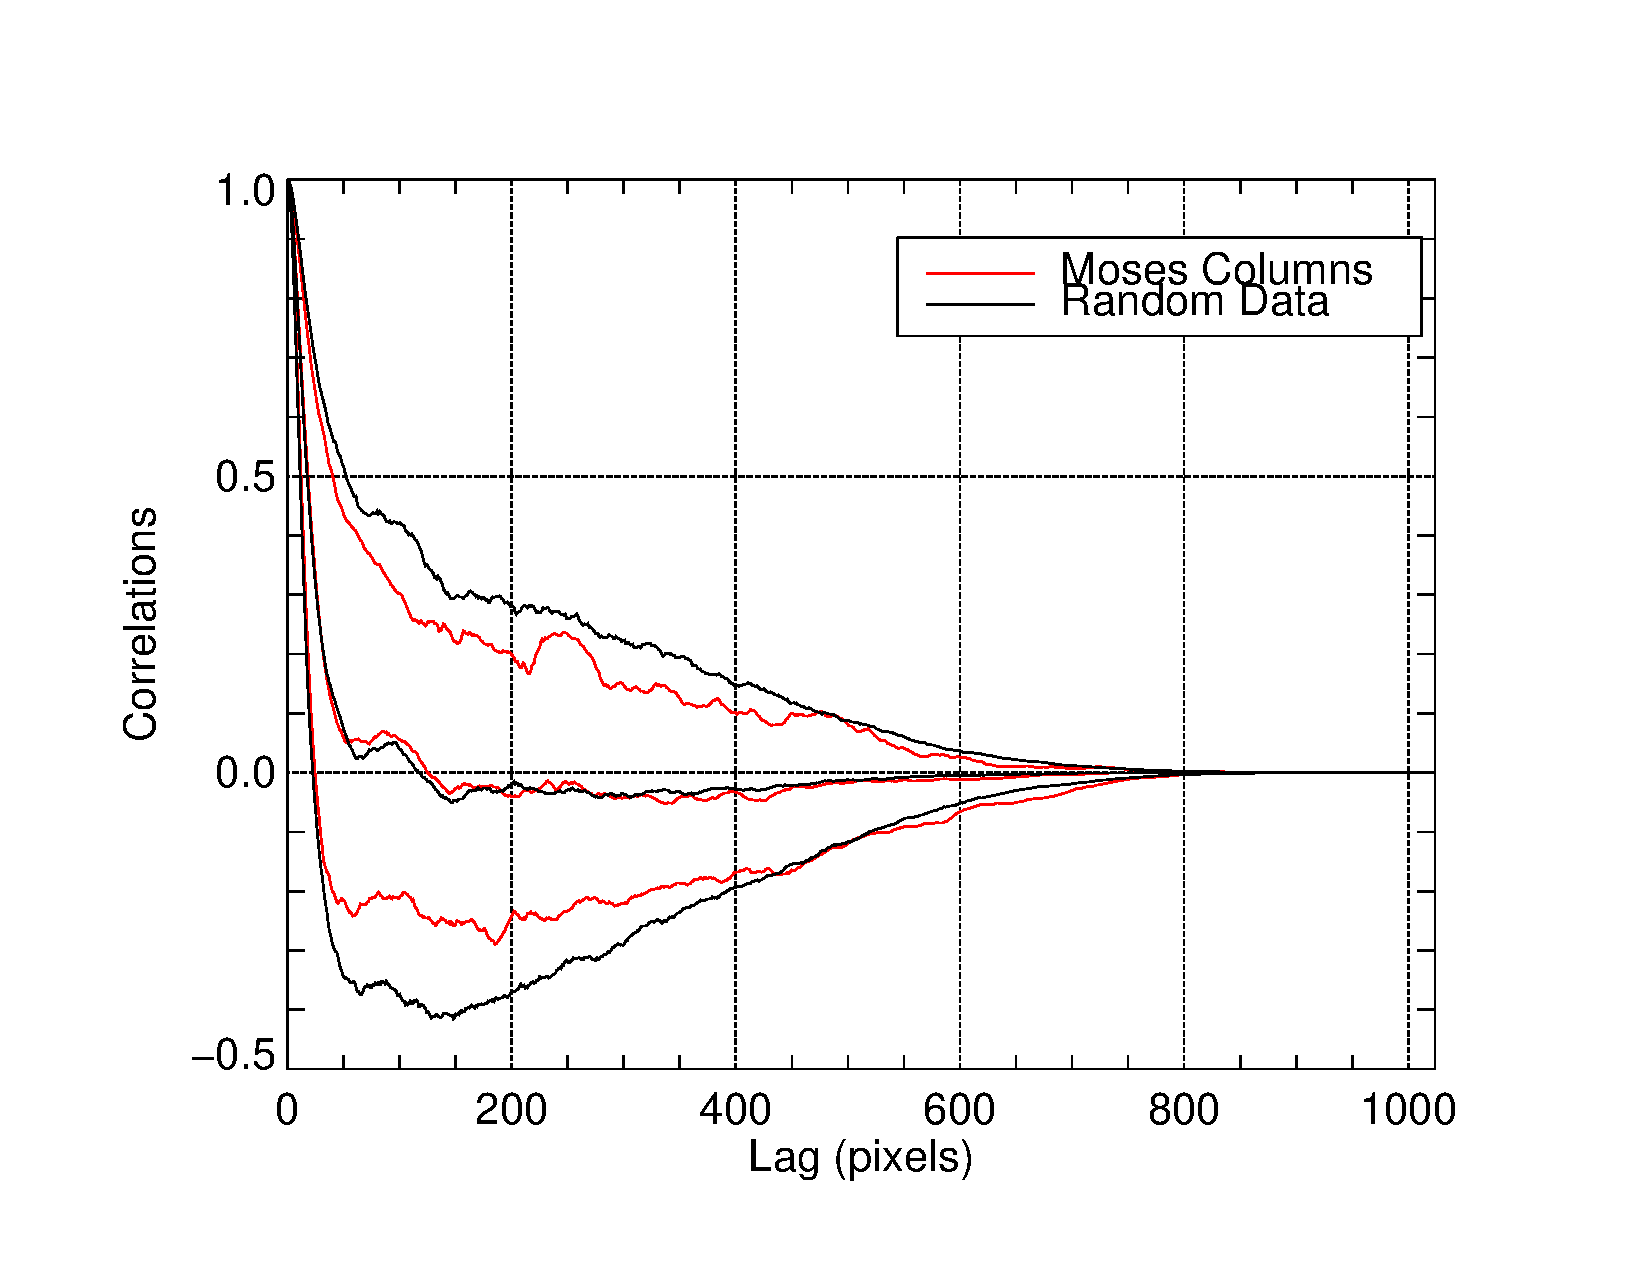
\includegraphics[width=\linewidth]{images/sigtestauto}
		\caption{The 10th, 50th, and 90th percentile of the autocorrelation distribution for each value of k is plotted for both the MOSES columns and synthetic data.}
		\label{fig:sigtestauto}
	\end{figure}
	
	Figure \ref{fig:sigtest} shows the results of our significance testing with 10,000 synthetic arrays.  Each set of three arrays, $Z'$, $M'$ and $P'$, are subtracted and correlated according to Equation \ref{eqn:cross_correlate}. The 99.99\% confidence interval is found by removing a percentage, $p$, from either end of the distribution for each lag and is found through the following equation:
	
	\begin{equation}
	.9999 = 1-(2p)^n.
	\end{equation}
	Here n is the number of degrees of freedom in the system or number of independent MOSES rows being cross-correlated.  By picking a confidence level and a representative n we determine what percentage of data, p, is outside the confidence interval.  A good indication of the value of n is the autocorrelation length (the lag at which autocorrelation falls to zero and begins random oscillation) of the MOSES columns.  Figure \ref{fig:sigtestauto} shows that the correlation length is any where from 50 to 150 pixels. This implies that there are anywhere from 7-20 unique MOSES rows.  The significance curves in Figure 5 were plotted using a conservative n=5. 
	
	We find that the mean cross-correlation of MOSES difference images along their rows has peaks that are much greater than the 99.99\% confidence interval and are therefore significant and indicative of extra spectral content. 
	
	\cck{It may be worth discussing the properties of the synthetic rows in more detail. Not all of the following are necessarily important; somewhat in brainstorming mode here. Are the synthetic data positive definite? Does it matter (probably not)? Do the rows show similar power spectra? How might the synthetic data may differ from the real thing, in ways other than the spectral lines we are looking for? For example, there are also line profile and PSF effects. This could change the structure near zero lag, but the effective range of these features is probably small (how many pixels?). } 
	
	
	\subsection{Forward Model} 
	The mean cross-correlation of MOSES difference image rows is shown in Figure \ref{fig:sigtest}.  In Section \ref{sec:sigtesting} several peaks in correlation were deemed to be significant and indicative of extra spectral content in the MOSES  data.  These peaks have irregular, broad profiles and are both positive and negative.  To interpret how these peaks in correlation relate to spectral content we developed a forward model that produces synthetic MOSES difference images with known spectral content using Chianti \citep{} and images from EIT \citep{}.  
	

	\subsection{Fitting}
	Using a MCMC to thoroughly explore the parameter space and generate error bars on fit parameters. More work to be done here.

\section{Results}
	Synthetic images of best fit.  Quantify extra spectral content.  Comment on extra He II emission unaccounted for by Chianti. 

\section{Discussions/Conclusions}
	Implications for future, design changes incorporated in ESIS (field stop, line selection, dispersion increase?). Possibly examine the spectra surrounding Ne VII 465 \AA.  Do we have the MOSES II throughput curves? 
	
\bibliography{ParkerKankelborg2018}

\section{Acronyms}
	\begin{acronym}
		\acro{MOSES}{Multi-Order Solar EUV Spectrograph}
		\acro{EIT}{EUV Imaging Telescope}
		\acro{SOHO}{Solar and Helioshperic Observatory}
	\end{acronym}


\end{article}
\end{document}
	
